\documentclass[tikz, convert={convertexe=magick}, png]{standalone}

\usepackage[compat=0.4]{yquant}
\usepackage{braket}
\yquantset{register/default name=$\ket{\reg_{\idx}}$}

\begin{document}
   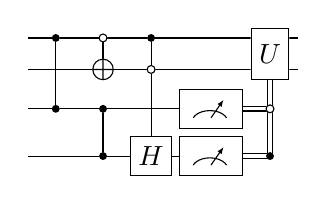
\begin{tikzpicture}
      \begin{yquant*}
         zz (a[0, 2]);
         cnot a[1] ~ a[0];
         zz (a[2, 3]);
         h a[3] | a[0] ~ a[1];
         measure a[2, 3];
         box {$U$} (a[0, 1]) | a[3] ~ a[2];
         discard a[2, 3];
      \end{yquant*}
   \end{tikzpicture}
\end{document}